\newpage{}
\section{Problema C: Construyendo murallas}
\textbf{Peso del ejercicio: 10}

\subsection{Descripción del problema}
% intro, contar que onda
Se nos dan $H$ puntos que representan lugares históricos de un reino, 
y otros $E$ puntos que representan edificios de un reino enemigo. 

Se quieren encerrar dentro de una muralla algunos puntos de los lugares históricos, 
con las condiciones de que no quede ningún punto enemigo dentro de la muralla, 
y que la muralla debe ser un polígono convexo. Además queremos maximizar la cantidad 
de lugares históricos que quedan dentro de la muralla. \\

Por ejemplo, si en la figura los puntos con marcados con círculos azules son lugares históricos 
y los marcados con cuadrados rojos son edificios enemigos, la solución óptima estaría dada por 
el polígono marcado con líneas, cuyo valor sería 4. 
% TODO dibujito con ejemplo 

\begin{center}
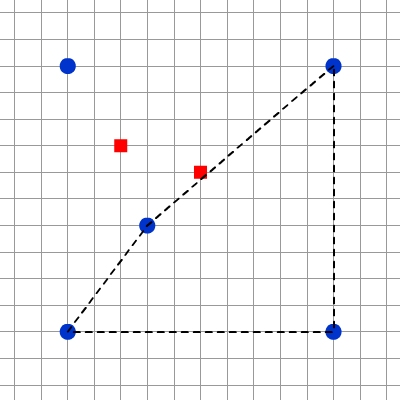
\includegraphics[width=0.35\textwidth]{ej3_1.jpg}
\end{center}

Siendo $N = H + E$, se nos pide encontrar un algoritmo que sea polinomial, en el mejor 
de los casos con complejidad temporal $O(N^5)$ u $O(N^4)$. Se asume además que no existirán 
tres puntos alineados en la entrada. \\

\textbf{Solución propuesta}

La solución que proponemos tiene complejidad temporal de $O(N^4)$, se basará fuertemente 
en la utilización de triángulos. Para empezar, enunciamos algunas propiedades y observaciones 
útiles que serán importantes para entender la solución. 

\subsection{Observaciones importantes}
% triangulacion, triangulos faciles
\begin{itemize}
\item El polígono que debemos hallar es un polígono convexo, sabemos que todo 
polígono convexo admite una triangulación. En particular, también admite una triangulación 
en la que todos las diagonales salen de un mismo vértice. Llamaremos a este vértice \textit{pivote} 
para futuras referencias. 
\item Dados tres puntos (y asumiendo que no habrá 3 puntos alineados), es unívoco el triángulo que se 
forma y además no será degenerado nunca. El hecho de que sea unívoco no es cierto para polígonos más 
grandes, y además hará más simple el algoritmo. 
\item Queremos además encontrar un polígono convexo que contenga la mayor cantidad de puntos \textit{buenos} 
(los lugares históricos) y que no incluya ningún punto \textit{malo} (los edificios enemigos). 
Dado un triángulo, y otro punto (que no sea ninguno de sus vértices), es fácil verificar si el punto 
cae dentro o fuera del triángulo (más adelante daremos detalles de esto). Esta información y el 
hecho que sea simple, nos ayudarán con el algoritmo. 
\end{itemize}

\subsection{Explicación del algoritmo}
Usando estas observaciones construiremos nuestro algoritmo. La idea del mismo tiene elementos similares 
con el algoritmo de Graham para hallar una cápsula convexa dados un conjunto de puntos. 

La idea será tratar de ir formando polígonos convexos en base a triángulos, que como vimos forman 
una buena descomposición del polígono y simplifican varias cuestiones de cálculo geométrico. \\

\textbf{Preproceso}

Primero lo que haremos será tomar todos los triángulos formados por tres puntos buenos distintos, 
y para cada uno calcular cuántos otros puntos buenos caen dentro del triángulo y si cae algún punto malo 
también. Guardaremos esta información para cada triángulo, dado que luego la utilizaremos en 
el cálculo de la solución. Llamaremos \textit{puntaje} de un triángulo a la cantidad de puntos buenos 
que caigan dentro del triángulo, y diremos que un triángulo es \textit{válido} si no tiene 
ningún punto malo en su interior. 

Iterar sobre todos los triángulos formados por puntos buenos tiene complejidad 
$O(N^3)$ y se puede computar en tiempo constante si un punto cae dentro de un triángulo (más adelante 
explicaremos cómo). 
De modo que todo este preproceso puede hacerse en $O(N^4)$.\\

\textbf{Cálculo de la solución}

Tomamos un punto cualquiera que supondremos será el \textit{pivote} 
del polígono de nuestra solución. Con el resto de los puntos, trateremos de formar polígonos 
convexos usando triángulos que usen el \textit{pivote} como vértice. Como tenemos fijo uno 
de los puntos (el \textit{pivote}) hay en total $O(N^2)$ triángulos sobre los que iterar. 
Para facilitar el chequeo de que los polígonos resultantes sean convexos, 
sólo tomaremos puntos que se encuentren más arriba que el \textit{pivote}.

Entonces, el algoritmo va recorriendo los triángulos (o bien, los 2 puntos que formarían el triángulo 
con el \textit{pivote}) en orden según el ángulo que forman con el \textit{pivote}. De esta forma, 
se puede plantear un algoritmo de programación dinámica que calcula, para cada triángulo $T$ que 
usa el \textit{pivote}: cuál es el mejor puntaje acumulado que se puede lograr armando 
un polígono convexo (y sin puntos malos), si el último triángulo que se agrega al polígono 
es $T$. Llamamos a este valor \texttt{dp[T]}.

Para calcular esto para todo triángulo $T$, debemos tener calculado previamente también 
\texttt{dp[T']} para los $T'$ triángulos que se encuentren antes según el ángulo con el 
\textit{pivote}, donde $T'$ sería el anteúltimo triángulo del polígono (justo antes que $T$). 
Es por esto que recorremos los triángulos en orden en algún sentido (horario u 
antihorario), cuando querramos calcular \texttt{dp[T]} tendremos calculado ya el valor de los triángulos 
anteriores. 

Es claro que como $T'$ debe ir inmediatamente antes que $T$, no cualquier triángulo puede 
servir como $T'$, debe cumplir entonces que: 
\begin{itemize}
\item $T'$ debe ser \textit{adyacente} a $T$, en el sentido que debe compartir un lado, de manera 
que los triángulos se ``peguen bien''. Dicho de otra forma, si $T$ está formado por los puntos $i$ y $j$ 
(con $i$ antes que $j$ según el \textit{pivote}), entonces $T'$ debe estar formado por $k$ e $i$ 
(con $k$ antes que $i$). 
\item Siempre los triángulos que miramos, tanto $T$ como $T'$ deben ser \textit{válidos} (no 
contener puntos malos). 
\item Se debe mantener la convexidad del polígono. Para esto, basta con mirar (similar a cómo 
funciona el algoritmo de Graham) que los puntos $k$, $i$ y $j$ formen un ángulo convexo (menor a 180 grados). 
De esta forma (y además, como los puntos estaban por debajo del \textit{pivote}), 
todos los ángulos interiores del polígono resultante serán menores a 180 grados, y 
por tanto el polígono será convexo. 
\end{itemize}

% TODO dibujo aqui con explicacion
Mostramos a continuación un par de figuras para tratar de aclarar cómo funcionaría 
el algoritmo. El punto marcado con una $P$ sería el pivote en este caso, el triángulo 
marcado con líneas fuertes sería en el que estamos parados, y los triángulos con líneas punteadas 
son los triángulos adyacentes a este. 

\begin{center}
\begin{tabular}{cc}
  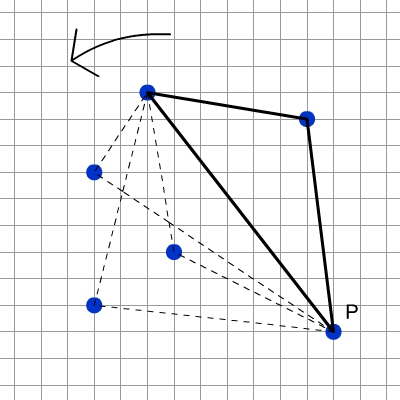
\includegraphics[width=0.35\textwidth]{ej3_2.jpg} &

  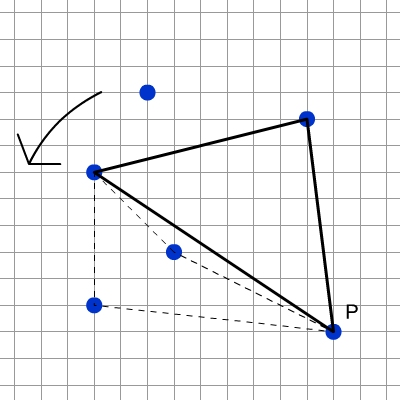
\includegraphics[width=0.35\textwidth]{ej3_3.jpg}
\end{tabular}
\end{center}

\subsection{Pseudocódigo}

En el preproceso calculamos para cada triángulo si es válido, y su puntaje. 

\begin{algorithm}[H]
\caption{Preproceso}
\For{\textbf{each} terna $[i,j,k], i,j,k \in puntosBuenos$}{
  \If{$i,j,k$ son distintos}{
    $T \leftarrow$ triangulo formado por $[i,j,k]$\;
    \For{\textbf{each} $p \in puntosMalos$}{
      \If{$p$ cae dentro de $T$}{
        marcar $T$ como no valido\;
      }
    }
    \For{\textbf{each} $p \in puntosBuenos$}{
      \If{$p$ cae dentro de $T$}{
        puntaje[$T$]++\;
      }
    }      
  }
}
\end{algorithm}

Luego calculamos la solución iterando sobre los distintos pivotes. 
Cuando tengamos $H \geq 2$, la respuesta será mínimo 2 porque al no haber 
3 puntos alineados, existirá un polígono lo suficientemente chico que contenga 
2 puntos buenos sin ninguno malo. Analogamente, siempre puede hacerse un polígono 
con 1 solo punto bueno. Por esto, al principio del algoritmo, tomamos $R$ (la respuesta) 
como el mínimo entre 2 y $H$. 

\begin{algorithm}[H]
\caption{Cálculo de la solución}
$R \leftarrow min(2,H)$\;
ordenar $puntoBuenos$ por coordenada $Y$ y luego coordenada $X$\;
\For{\textbf{each} $pivot \in puntosBuenos$}{
  $S \leftarrow$ puntos que están luego de $pivot$\;
  ordenar $S$ por ángulo respecto de $pivot$\;
  \For{\textbf{each} $i \in S$}{
    \For{\textbf{each} $j \in S, j > i$}{
      $T \leftarrow$ triangulo formado por $[pivot,i,j]$\;
      \If{$T$ es válido}{
        \For{\textbf{each} $k \in S, k > j$}{
          $U \leftarrow$ triangulo formado por $[pivot,j,k]$\;
          \If{$U$ es válido $\wedge$ $i,j,k$ forman un ángulo convexo}{
            marcar $U$ y $T$ como adyacentes\;
          }
        }
      }
    }
  }
  \For{\textbf{each} $i \in S$}{
    \For{\textbf{each} $j \in S, j > i$}{
      $T \leftarrow$ triangulo formado por $[pivot,i,j]$\;
      \If{$T$ es válido}{
        dp[$T$] $\leftarrow$ puntaje[$T$] + 3\;
        \For{\textbf{each} $k \in S, k < i$}{
          $U \leftarrow$ triangulo formado por $[pivot,k,i]$\;
          \If{$T$ y $U$ son adyacentes}{
            dp[$T$] $\leftarrow max$(dp[$T$], dp[$U$] + puntaje[$T$] + 1)\;
          }
          $R \leftarrow max(R, $dp[$T$]$)$\;
        }
      }
    }
  }
}
\end{algorithm}

\textbf{Correctitud del algoritmo}

La solución al problema será el mayor puntaje de algún polígono convexo, 
en particular por lo que vimos antes, este polígono puede tener un pivote y puede 
ser cualquiera de sus vértices (en particular, el de más abajo como elegimos nosotros). 

Además, este polígono siempre admitirá una triangulación respecto de ese pivote, y como 
estamos considerando en la dinámica a todos los triángulos posibles salientes de ese pivote, entonces 
siempre podremos obtener la mejor solución para un pivote dado. 

Como no podemos saber a priori cuál de los puntos buenos será el verdadero pivote de la solución, 
probamos con todos, de esta forma cubirmos todas las soluciones posibles. 

\subsection{Detalles sobre el algoritmo/implementación}
\begin{itemize}
\item Para chequear que el ángulo formado por 3 puntos sea un ángulo convexo, usamos 
el producto cruz, al igual que en el algoritmo de Graham para hallar la cápsula convexa. 
Hacer este cálculo lleva tiempo constante. 
\item Todos los puntos tienen coordenadas enteras, de modo que sus valores, y 
las operaciones que necesitamos hacer con ellos (producto cruz, norma cuadrado) puede almacenarse 
en enteros. 
\item Para ordenar los puntos por ángulo formado con el pivote, también utilizamos el producto 
cruz. 
\item Para calcular si un punto $p$ está contenido en un triángulo $(i,j,k)$, lo que hacemos 
es calcular el sentido (horario o antihorario) en el que están dispuestos los conjuntos de puntos 
$(p,i,j)$, $(p,j,k)$ y $(p,k,i)$. Si y solo si los tres cálculos dan el mismo resultado, quiere 
decir que $p$ debe estar contenido en el triángulo. Para saber si la disposición es horario o antihoraria, 
nuevamente usamos el producto cruz. Podemos ver entonces que chequear si punto cae dentro de un triángulo 
puede hacerse en tiempo constante de esta forma. 
\end{itemize}
% diferencia entre N^4 y N^5, como hacerlo 
% explicar el bind? 
% que los puntos tienen coordenadas enteras nomas
% punto en triangulo 

\subsection{Análisis de complejidad}
% ganar
Podemos ver en base a los pseudocódigos, y dado que ya vimos que chequear ángulos 
o pertenecia de un punto en un triángulo lleva tiempo constante, que todo el preproceso 
del algoritmo tiene complejidad $O(N^4)$, porque iteramos sobre todas las ternas de puntos que son 
$O(N^3)$ y para cada una vemos para cada punto $p$ si cae dentro del triángulo formado por la terna. 

Luego iteramos sobre todos los pivotes, que en total son $O(N)$, ordenamos un conjunto de puntos 
según el ángulo que forman con el pivote (como mucho son $O(N)$, por tanto esto puede hacerse 
en $O(N log N)$). Como vimos, fijado el pivote, dados otros 2 puntos, estos forman un triángulo, 
entonces para cada pivote hay $O(N^2)$ triángulos, además para cada uno, debemos ver cuáles triángulos 
adyacentes a este, y usar sus soluciones para la dinámica. Como los triángulos adyacentes deben compartir 
2 puntos (el pivote y otro más), hay en total $O(N)$ puntos para probar para los triángulos adyacentes. 

El cálculo de la solución es entonces: $O(N) * O(N log N) * O(N^2) * O(N) = O(N^4)$. 

Podemos ver entonces que todo el algoritmo tiene complejidad $O(N^4)$. 

\newpage
\subsection{Código de la solución}
\lstinputlisting[numbers = left]{../src/ej3/ej3.cpp}
